% !TEX root = ../my_thesis.tex

\section{Ergebnisse}
Im vorliegenden Kapitel werden die Ergebnisse der durchgeführten Experimente präsentiert. In dieser Arbeit gibt ein Evaluationsergebnis eines Netzwerkes die Abweichung der Position in Metern sowie Orientierung in Grad an und der Median der Evaluationsergebnisse bestimmt die Akkuratesse eines KNNs. Somit bildet sich die Akkuratesse eines Netzwerkes aus der Zusammensetzung von Positions- sowie Orientierungsfehler. In dieser Arbeit wird ein Evaluationsergebnis und eine Akkuratesse gegenüber Seinesgleichen anhand des Positionsfehlers verglichen.

Im weiteren Verlauf dieses Kapitels werden zuerst die Reproduktionsergebnisse von BIM-PoseNet \cite{acharyaBIMPoseNetIndoorCamera2019} angegeben. Anschließend werden die Evaluationsergebnisse der trainierten Netzwerke angezeigt.

\subsection{Reproduktion der Ergebnisse von BIM-PoseNet}
Die Ergebnisse der Experimente von \citet{acharyaBIMPoseNetIndoorCamera2019}, die das PoseNet Model mit Gradientenbilder der karikaturistischen Daten (\textit{grad-cartoon}) sowie synthetischen Kantenbilder trainierten (\textit{grad-edge}) und anschließend mit den Gradientenbildern der realen Daten (\textit{grad-real}) evaluierten, konnten näherungsweise (vgl. Tab. \ref{tab:reproduction}) reproduziert werden. Abweichend von BIM-PoseNet wurden statt 1000 reale Bilder, 600 reale Bilder evaluiert, weil zu derzeit 600 Evaluierungsbilder veröffentlicht waren. Der Trainingsprozess wurde pro Datensatztyp 5-mal wiederholt und die bessere Akkuratesse wurde behalten. Eine exakte oder bessere Reproduktion der Ergebnisse ist durch Zufall bedingt und wurde in dieser Arbeit aus Zeitgründen vernachlässigt. Tabelle \ref{tab:reproduction} präsentiert die Ergebnisse der Reproduktion sowie die Ergebnisse der Autoren \citet{acharyaBIMPoseNetIndoorCamera2019}.


\begin{table}[b]
	\centering
	\caption{Reproduktionsergebnisse. Abweichungen der Ergebnisse sind durch Zufall bedingt und können bei mehrfachem Wiederholen des Trainingsprozesses minimiert bzw. erhoben sowie verbessert werden. }
	\begin{tabularx}{1.0\textwidth}{X X X}
		\textbf{Trainingsdatensatz} \hspace{2cm} (Gradientenbild) & \textbf{BIM-PoseNet} \hspace{2cm} (Position, Orientierung) & \textbf{Reproduktion} \hspace{2cm} (Position, Orientierung)\\
		\hline
	 \textit{grad-cartoon} & 2.63$m$, 6.99° & 2.57$m$, 10.52°\\
		\hline
		\textit{grad-edge} & 1.88$m$, 7.73°  & 2.53$m$, 9.54°\\
	\end{tabularx}
	\label{tab:reproduction}
\end{table}





\subsection{Evaluation der trainierten KNNs}
Für alle synthetischen Datensätze wurde separat das Trainingsprozess 5-mal mit den korrespondierenden Gradientenbildern der Trainingsdaten wiederholt. Eine Evaluierung folgte mit den Gradientenbildern der korrespondierenden synthetischen und realen Evaluationsdaten. Es wurden pro Strecke (s. Tab. \ref{tab:dataset_metrics}) und Datensatztyp nur die beste Akkuratesse behalten. Tabelle \ref{tab:results_ic} bis \ref{tab:results_hs_stairs_down} geben die Akkuratesse der KNNs auf den jeweiligen Strecken an. 

Für ein besseres Verständnis der durch die Evaluierung mit den \textit{grad-real} Datensätzen resultierenden Akkuratessen wurden für die KNNs mit der besten Akkuratesse pro Strecke die bestimmten Positionen in der xy-Ebene dargestellt. Ebenso wurden pro Strecke der Positionsfehler in der xy-Ebene und der Orientierungsfehler auf der Gierachse der jeweiligen Evaluationsdaten dargestellt. Abbildungen \ref{fig:result_ic_loop} bis \ref{fig:result_hs_stairs_down} illustrieren die Evaluationsergebnisse.


\subsubsection{IC-loop}
% die eine geschlossen Schleife in einem optisch ähnlichen Flur bildet,
%  der Ansatz von \citet{acharyaBIMPoseNetIndoorCamera2019} auf einer ebenen, gegen den UZS abwechselnde Richtung verlaufenden, ca. 115$m$ langen Strecke mit wiederholenden Gebäudemerkmalen 
% Alle Datensätze der Strecke \textit{IC-loop} wurden zu 50\% Trainingsdaten und zu 50\% Evaluierungsdaten zufällig aufgeteilt. Für alle synthetischen Datensatztypen mit je 5718 Daten wurde ein separates Netzwerk trainiert. Anschließend wurden die Netzwerke mit den korrespondierenden synthetischen Evaluierungsdatensätze mit je 5717 Daten getestet. Eine weitere Evaluierung der trainierten Netzwerke folgte mit den realen 1921 Evaluierungsdaten. Tabelle \ref{tab:results_ic} gibt die Ergebnisse dieser Evaluierungsvorgänge an.
% Aus Tabelle \ref{tab:results_ic} ist zu erkennen,

In diesem Experiment wurde der \textit{IC-loop} Datensatz verwendet. 
Mit ausschließlich synthetischen Daten beim Trainieren und Evaluieren konnte eine Akkuratesse von 1.61$m$ in der Position und 8.17° in der Orientierung durch den \textit{grad-cartoon} Datensatz erzielt werden (vgl. Tab. \ref{tab:results_ic}). Dies zeigt die potenzielle Fähigkeit des Experimentes zur Pose Estimation auf der \textit{IC-loop} Strecke bei Daten derselben Domäne. 

Bei der Evaluierung mit den Gradientenbildern der realen Evaluationsdaten konnte auf dem mit \textit{grad-photoreal} trainiertem Netzwerk eine Akkuratesse von 16.68$m$ in der Position und 73.25° in der Orientierung erreicht werden (vgl. Tab. \ref{tab:results_ic}). Bei einem Gebäudevolumen von ca. $50m \times 11m \times 3.5m$ ist die Positionsgenauigkeit von 16.68$m$, mit Anbetracht des Abdriftens der realen Ground-Truth-Daten (s. Abschn. \ref{subsec:record_real_data}), für ein denkbares Lokalisierungsverfahren zu ungenau. Genauso ist eine Orientierungsgenauigkeit von 73.25° für die Bestimmung der Orientierung mehr als ungeeignet. Abbildung \ref{fig:result_ic_loop} visualisiert die Evaluierungsergebnisse von dem mit \textit{grad-photoreal} trainiertem sowie mit \textit{grad-real} evaluiertem Netzwerk.

In Abbildung \ref{subfig:ic_fig2} ist deutlich zu erkennen, dass das mit \textit{grad-photoreal} trainierte Netzwerk die Position aller \textit{grad-real} Evaluationsdaten verteilt auf einem ca. 30$m$ langen Teilbereich der unteren horizontalen Strecke bestimmt hat. Daher weisen Evaluationsdaten der kürzeren vertikalen sowie der obigen horizontalen Strecke die größten Positionsfehler auf (vgl. Abb. \ref{subfig:ic_fig4}). Ebenso kommt in Abbildung \ref{subfig:ic_fig6} hervor, dass das Netzwerk größtenteils die Orientierung der Evaluationsdaten als die Aufnahmerichtung der unteren horizontalen Strecke bestimmt hat. Offensichtlich war das Netzwerk auf der gesamten \textit{IC-loop} Strecke unfähig zur Pose Estimation.

\begin{table}
	\centering
	\caption{Evaluationsergebnisse von der Strecke \textit{IC-loop}. Es wird die Akkuratesse der mit den jeweiligen Trainingsdaten trainierten Netzwerke angegeben, die mit den korrespondierenden synthetischen Evaluationsdaten sowie jeweils mit den realen Evaluationsdaten evaluiert wurden.  }
	\begin{tabularx}{1.0\textwidth}{X >{\RaggedRight}X >{\RaggedRight}X}
	\textbf{Trainingsdatensatz} \hspace{2cm} (Gradientenbild) & \textbf{synthetische Daten} \hspace{2cm} (Position, Orientierung) & \textbf{reale Daten} \hspace{2cm} (Position, Orientierung)\\
	\hline
		\textit{grad-cartoon} & 1.61$m$, 8.17° & 23.56$m$, 51.30°\\
		\hline
		\textit{grad-edge} & 2.00$m$, 8.29° & 32.91$m$, 59.17°\\
\hline
		\textit{grad-photoreal} & 1.80$m$, 7.70° & 16.68$m$, 73.25°\\
	\end{tabularx}
	\label{tab:results_ic}
\end{table}



\begin{figure}
	\setlength\extrarowheight{-15pt}
	\centering
	\begin{tabularx}{1.0\textwidth}{>{\centering\arraybackslash}p{0.05\textwidth} X}
		\subcaption{} \label{subfig:ic_fig2} & \imagetop{ 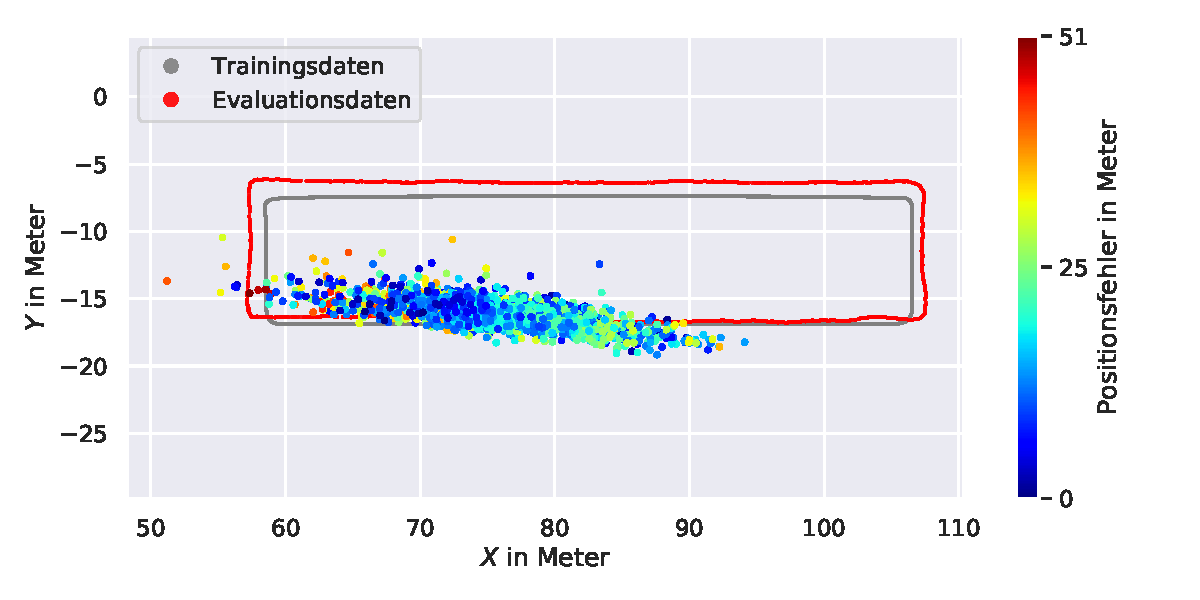
\includegraphics[width=1.0\linewidth]{images/results/ic_cycl/resultsfig_2.pdf} }\\
		\subcaption{} \label{subfig:ic_fig4} & \imagetop{ 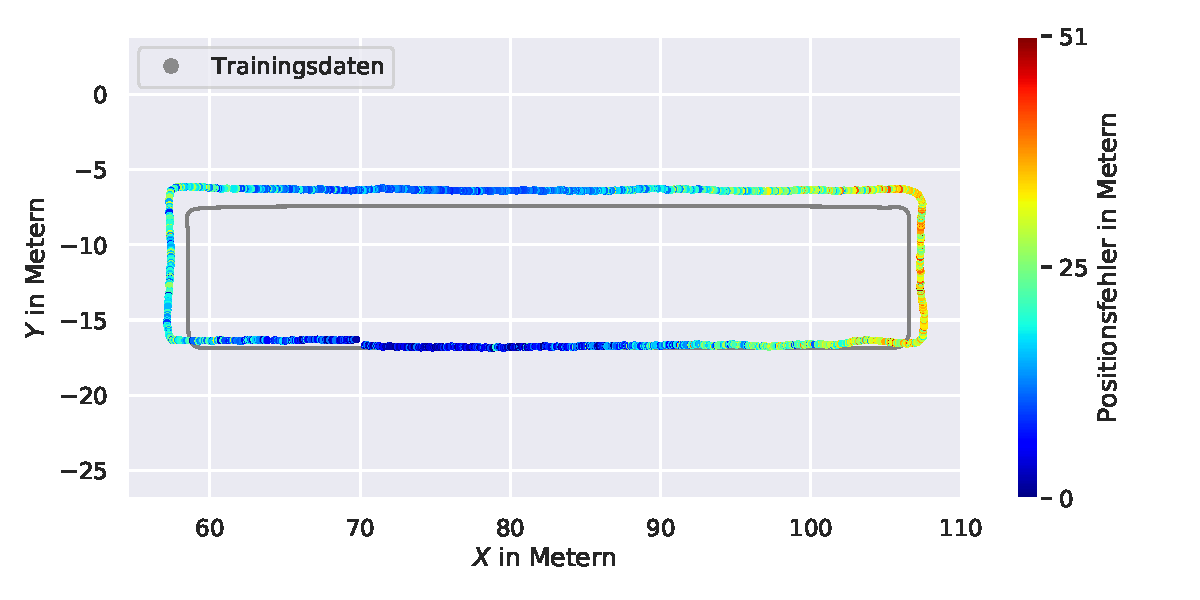
\includegraphics[width=1.0\linewidth]{images/results/ic_cycl/resultsfig_4.pdf} }\\
		\subcaption{} \label{subfig:ic_fig6} & \imagetop{ 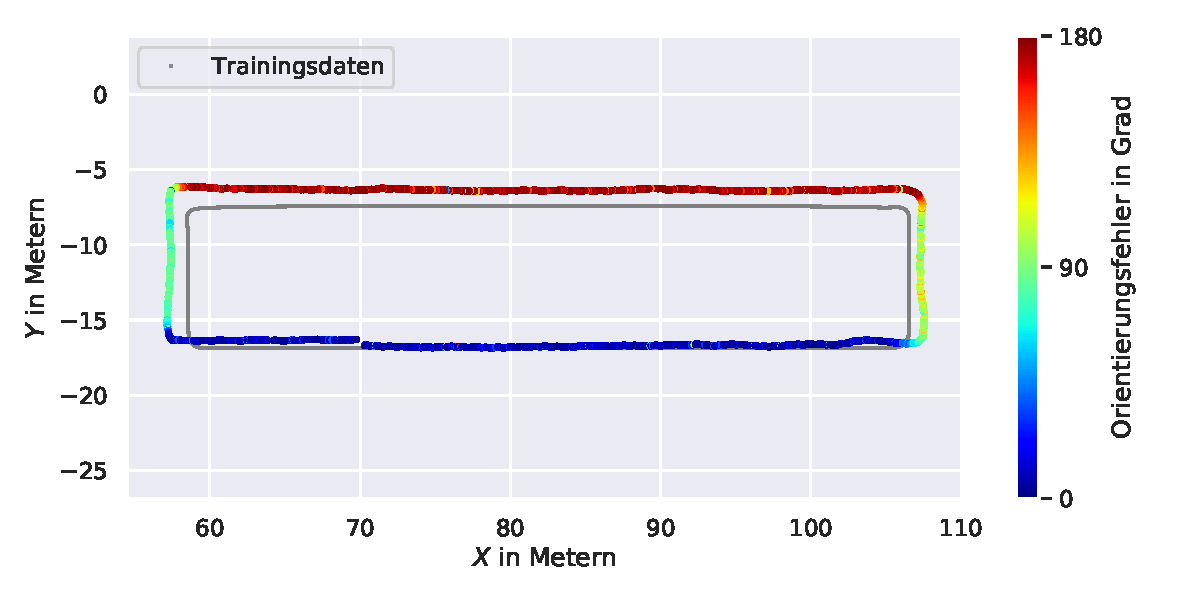
\includegraphics[width=1.0\linewidth]{images/results/ic_cycl/resultsfig_6.pdf} }\\
	\end{tabularx}
	\caption{Visualisierung der Evaluationsergebnisse von der Strecke \textit{IC-loop}. Die Evaluation folgte mit den Gradietenbildern der realen Daten auf das mit \textit{grad-photoreal} trainierten Netzwerk. \subref{subfig:ic_fig2} illustriert die Positionen auf der xy-Ebene, die von dem KNN bestimmt wurden. Der Positionsfehler in der xy-Ebene und der Orientierungsfehler auf der Gierachse der jeweiligen Evaluationsdaten werden in  \subref{subfig:ic_fig4} und  \subref{subfig:ic_fig6} dargestellt.}
	\label{fig:result_ic_loop}
\end{figure}


\subsubsection{HS-gamma}


Ein weiteres Experiment folgte mit den Datensätzen der \textit{HS-gamma} Strecke. Trainiert und Evaluiert mit nur synthetischen Daten konnte durch den \textit{grad-cartoon} Datensatz eine Akkuratesse von 1.00$m$ in der Position und 9.92° in der Orientierung erzielt werden (vgl. Tab. \ref{tab:results_hs_gamma}).  Dies stellt bei dem betroffenen Gebäudevolumen von $54m \times 10m \times 3m$ ein Potenzial zur Pose Estimation mit Daten der gleichen Beschaffenheit dar.

Die Evaluierung mit den \textit{grad-real} Evaluationsdaten auf dem mit \textit{grad-cartoon} trainiertem Netzwerk ergab eine Akkuratesse von 8.60$m$ in der Position und 19.59° in der Orientierung (vgl. Tab. \ref{tab:results_hs_gamma}). Bei oben genannten Gebäudemaßen ist eine Positionsgenauigkeit von 8.60$m$ sowie ein Orientierungsfehler von 19.59° unzureichend für die Bestimmung der Pose auf der \textit{HS-gamma} Strecke. Abbildung \ref{fig:result_hs_gamma} visualisiert die Evaluationsergebnisse von dem mit \textit{grad-cartoon} trainiertem und \textit{grad-real} evaluiertem Netzwerk.

Das mit \textit{grad-cartoon} trainierte Netzwerk bestimmte die Position aller \textit{grad-real} Evaluationsdaten auf ein ca. 20$m$ langem Teilbereich nahe der erwähnten Schleife im \textit{HS-gamma} Strecke (vgl. Abb.  \ref{subfig:hs_gamma_fig2}). Daher weisen Evaluationsdaten der kürzeren vertikalen sowie der obigen horizontalen Strecke die größten Positionsfehler auf (vgl. Abb\ref{subfig:ic_fig4}). Ebenso kommt in Abbildung \ref{subfig:ic_fig6} hervor, dass das Netzwerk größtenteils die Orientierung der Evaluationsdaten als die Aufnahmerichtung der unteren horizontalen Strecke bestimmt hat. Offensichtlich war das Netzwerk unfähig zur Pose Estimation in sich optisch ähnelnden Strecken.


\begin{table}
	\centering
	\caption{Evaluationsergebnisse von der Strecke \textit{HS-gamma}. Es wird die Akkuratesse der mit den jeweiligen Trainingsdaten trainierten Netzwerke angegeben, die mit den korrespondierenden synthetischen Evaluationsdaten sowie jeweils mit den realen Evaluationsdaten evaluiert wurden.}
	\begin{tabularx}{1.0\textwidth}{X >{\RaggedRight}X >{\RaggedRight}X}
	\textbf{Trainingsdatensatz} \hspace{2cm} (Gradientenbild) & \textbf{synthetische Daten} \hspace{2cm} (Position, Orientierung) & \textbf{reale Daten} \hspace{2cm} (Position, Orientierung)\\
	\hline
		\textit{grad-cartoon} & 1.00$m$, 9.92° & 8.60$m$, 19.59°\\
		\hline
		\textit{grad-edge} & 1.07$m$, 8.69° & 10.15$m$, 35.11°\\
		\hline
		\textit{grad-photoreal} & 1.45$m$, 9.17° & 10.27$m$, 41.60°\\
	\end{tabularx}
	\label{tab:results_hs_gamma}
\end{table}

\begin{figure}
	\setlength\extrarowheight{-15pt}
	\centering
	\begin{tabularx}{1.0\textwidth}{>{\centering\arraybackslash}p{0.05\textwidth} X}
		\subcaption{} \label{subfig:hs_gamma_fig2} & \imagetop{ 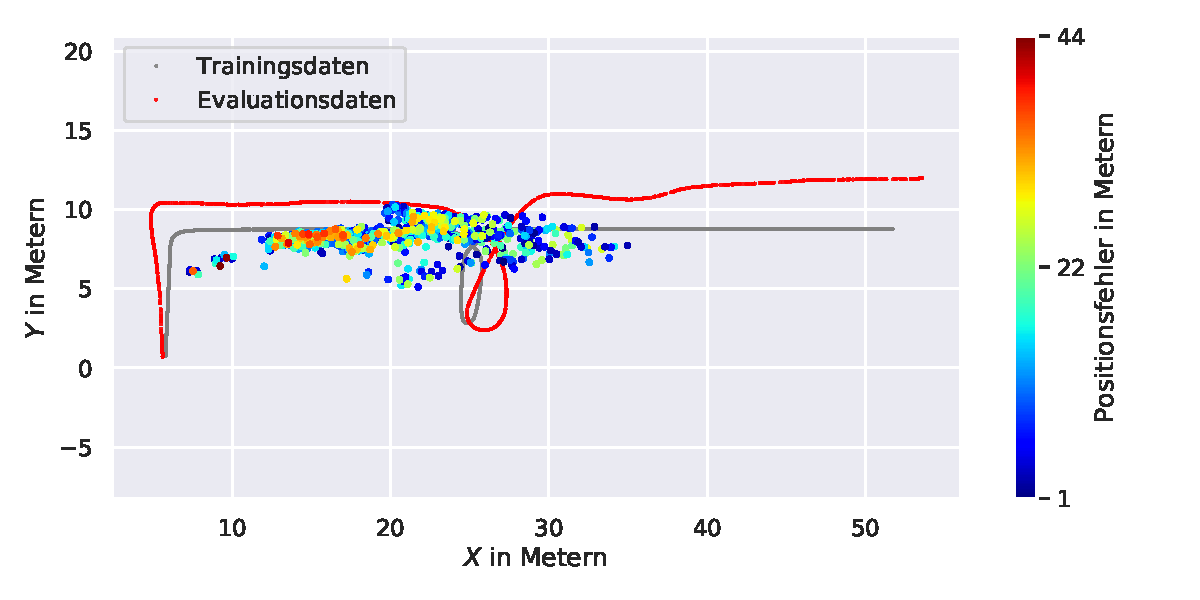
\includegraphics[width=1.0\linewidth]{images/results/hs_gamma/resultsfig_2.pdf} }\\
		\subcaption{} \label{subfig:hs_gamma_fig4} & \imagetop{ 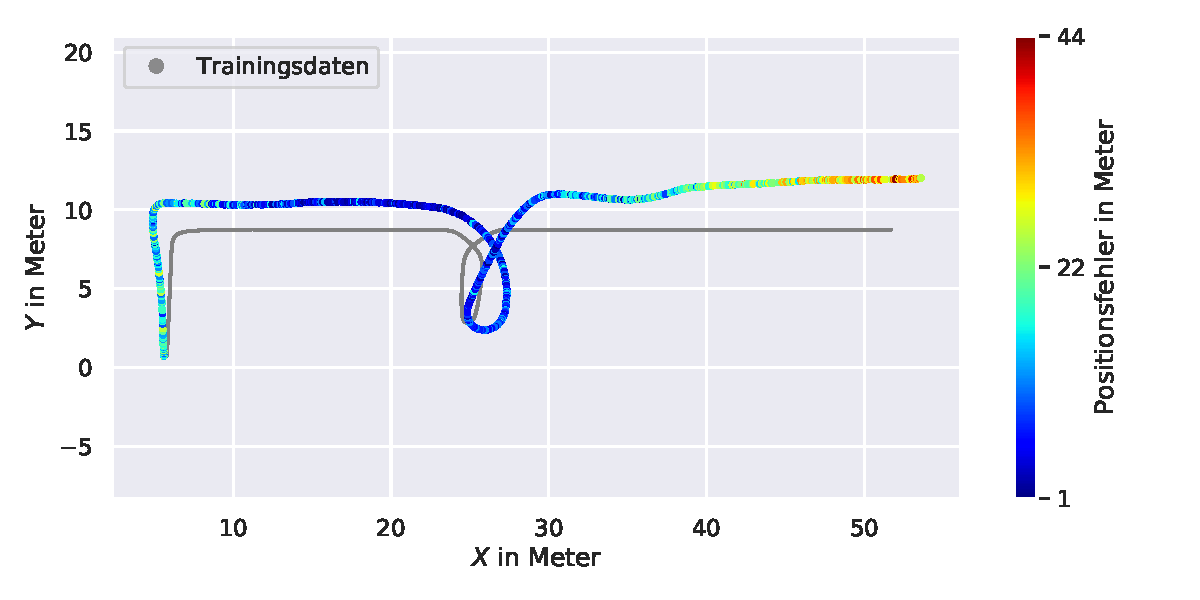
\includegraphics[width=1.0\linewidth]{images/results/hs_gamma/resultsfig_4.pdf} }\\
		\subcaption{} \label{subfig:hs_gamma_fig6} & \imagetop{ 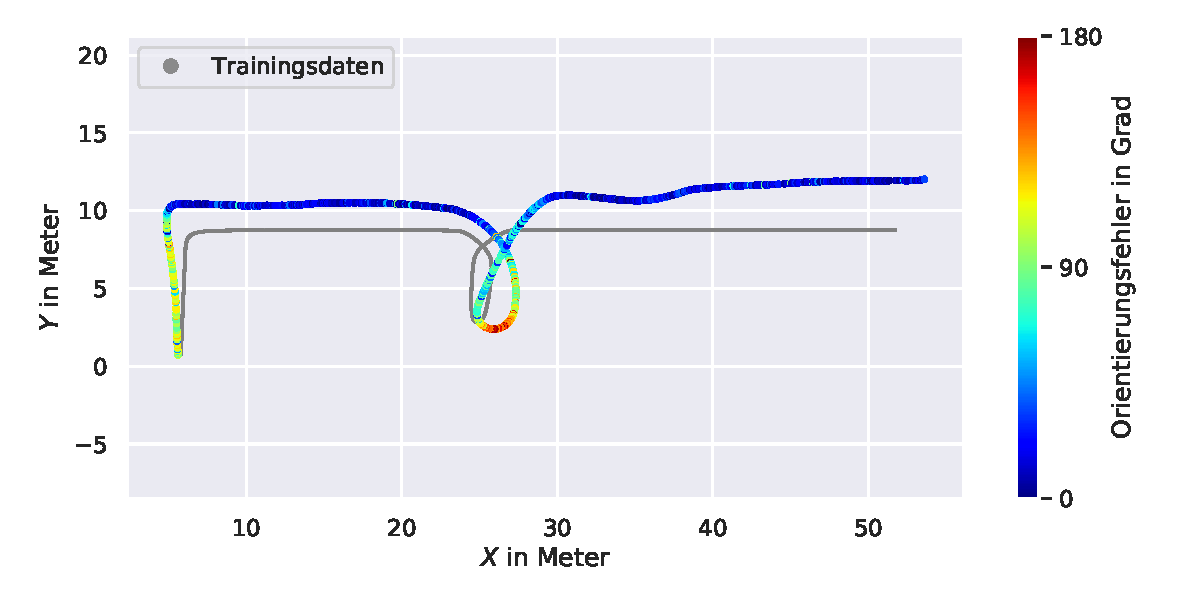
\includegraphics[width=1.0\linewidth]{images/results/hs_gamma/resultsfig_6.pdf} }\\
	\end{tabularx}
	\caption{Visualisierung der Evaluationsergebnisse von der Strecke \textit{HS-gamma}. Die Evaluation folgte mit den Gradietenbildern der realen Daten auf das mit \textit{grad-cartoon} trainierten Netzwerk. \subref{subfig:hs_gamma_fig2} illustriert die Positionen auf der xy-Ebene, die von dem KNN bestimmt wurden. Der Positionsfehler in der xy-Ebene und der Orientierungsfehler auf der Gierachse der jeweiligen Evaluationsdaten werden in  \subref{subfig:hs_gamma_fig4} und  \subref{subfig:hs_gamma_fig6} dargestellt.}
	\label{fig:result_hs_gamma}
\end{figure}

\subsubsection{HS-stairs-up}
Mit ausschließlich den Gradietenbilder der karikaturistischen Simulation konnte eine Akkuratesse von 0.82$m$ in der Position und 7.76° in der Orientierung erreicht werden. Bei der Evaluierung mit den Gradientenbildern der realen Daten konnte eine Akkuratesse von 4.33$m$ in der Position und 51.64° in der Orientierung auf dem Netzwerk erreicht werden, der mit den Gradietenbilder der synthetischen Kantenbildern trainiert wurde. Abbildung \ref{fig:result_hs_stairs_up} visualisiert die Evaluierungsergebnisse von diesem künstlichen neuronalen Netzwerk.
\begin{table}
	\centering
	\caption{Evaluationsergebnisse von der Strecke \textit{HS-stairs-up}. Es wird die Akkuratesse der mit den jeweiligen Trainingsdaten trainierten Netzwerke angegeben, die mit den korrespondierenden synthetischen Evaluationsdaten sowie jeweils mit den realen Evaluationsdaten evaluiert wurden.}
	\begin{tabularx}{1.0\textwidth}{X >{\RaggedRight}X >{\RaggedRight}X}
		\textbf{Trainingsdatensatz} \hspace{2cm} (Gradientenbild) & \textbf{synthetische Daten} \hspace{2cm} (Position, Orientierung) & \textbf{reale Daten} \hspace{2cm} (Position, Orientierung)\\
		\hline
		\textit{grad-cartoon} & 0.82$m$, 7.76° & 4.77$m$, 23.43°\\
		\hline
		\textit{grad-edge} & 0.82$m$, 8.48° & 4.33$m$, 51.64°\\
		\hline
		\textit{grad-photoreal} & 0.92$m$, 7.98° & 5.16$m$, 93.38°\\
	\end{tabularx}
	\label{tab:results_hs_stairs_up}
\end{table}


\begin{figure}
	\setlength\extrarowheight{-15pt}
	\centering
	\begin{tabularx}{1.0\textwidth}{>{\centering\arraybackslash}p{0.05\textwidth} X}
		\subcaption{} \label{subfig:hs_up_fig3} & \imagetop{ 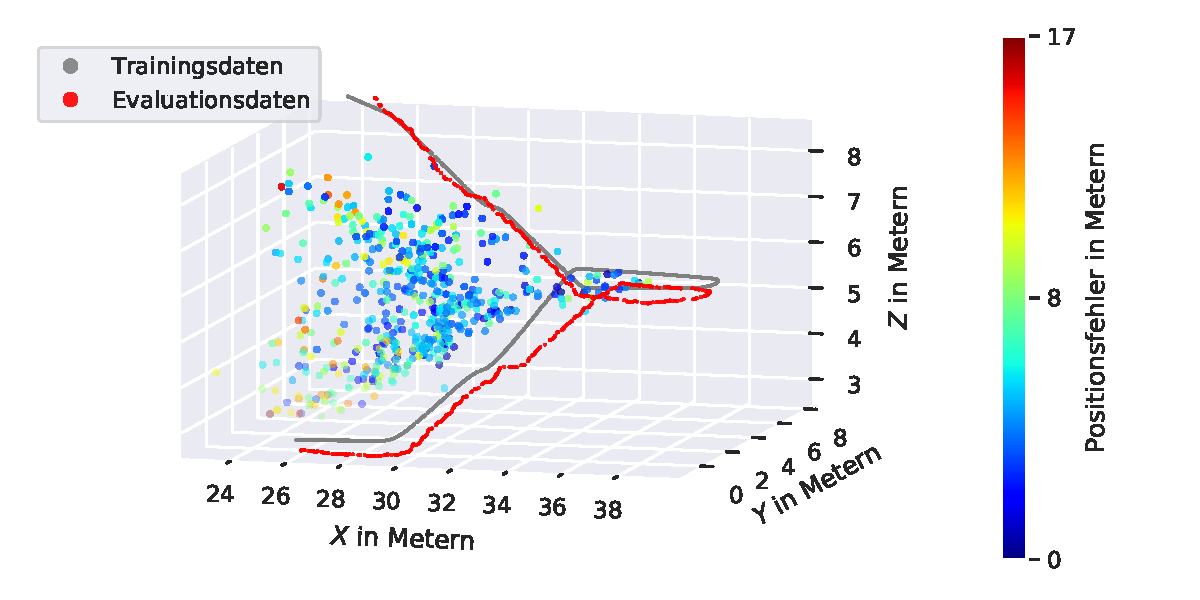
\includegraphics[width=1.0\linewidth]{images/results/hs_up/resultsfig_3.pdf} }\\
		\subcaption{} \label{subfig:hs_up_fig5} & \imagetop{ 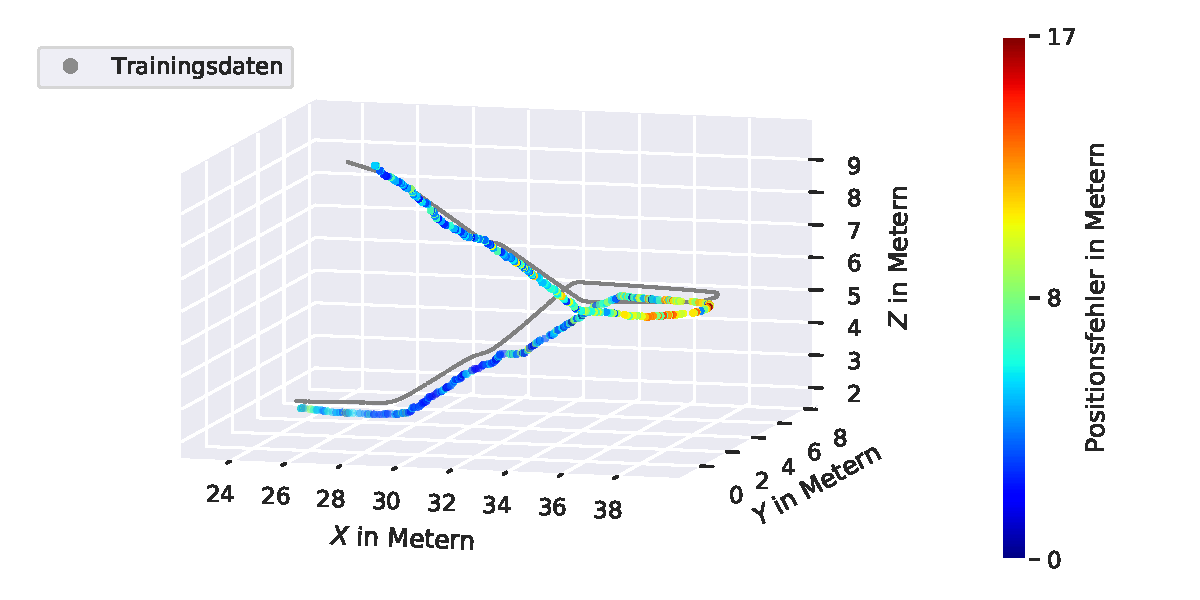
\includegraphics[width=1.0\linewidth]{images/results/hs_up/resultsfig_5.pdf} }\\
		\subcaption{} \label{subfig:hs_up_fig7} & \imagetop{ 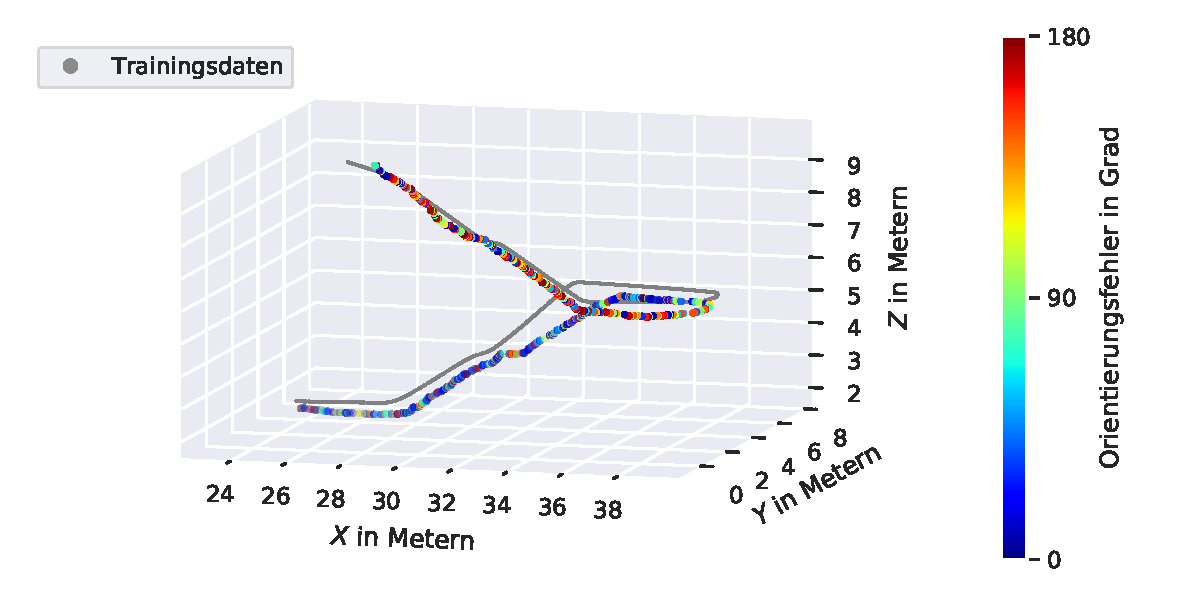
\includegraphics[width=1.0\linewidth]{images/results/hs_up/resultsfig_7.pdf} }\\
	\end{tabularx}
	\caption{Visualisierung der Evaluationsergebnisse von der Strecke \textit{HS-stairs-up}. Die Evaluation folgte mit den Gradietenbildern der realen Daten auf das mit \textit{grad-edge} trainierten Netzwerk. \subref{subfig:hs_up_fig3} illustriert die Positionen auf der xy-Ebene, die von dem KNN bestimmt wurden. Der Positionsfehler in der xy-Ebene und der Orientierungsfehler auf der Gierachse der jeweiligen Evaluationsdaten werden in  \subref{subfig:hs_up_fig5} und  \subref{subfig:hs_up_fig7} dargestellt.}
	\label{fig:result_hs_stairs_up}
\end{figure}


\subsubsection{HS-stairs-down}
 Mit ausschließlich den Gradietenbilder der synthetischen Kantenbildern konnte eine Akkuratesse von 0.85$m$ in der Position und 7.50° in der Orientierun erreicht werden. Bei der Evaluierung mit den Gradientenbildern der realen Daten konnte eine Akkuratesse von 4.20$m$ in der Position und 47.83° in der Orientierung auf dem Netzwerk erreicht werden, der mit den Gradietenbilder der karikaturistische Simulation trainiert wurde. Abbildung \ref{fig:result_hs_stairs_down} visualisiert die Evaluierungsergebnisse von diesem künstlichen neuronalen Netzwerk.
\begin{table}
	\centering
	\caption{Evaluationsergebnisse von der Strecke \textit{HS-stairs-down}. Es wird die Akkuratesse der mit den jeweiligen Trainingsdaten trainierten Netzwerke angegeben, die mit den korrespondierenden synthetischen Evaluationsdaten sowie jeweils mit den realen Evaluationsdaten evaluiert wurden.}
	\begin{tabularx}{1.0\textwidth}{X >{\RaggedRight}X >{\RaggedRight}X}
		\textbf{Trainingsdatensatz} \hspace{2cm} (Gradientenbild) & \textbf{synthetische Daten} \hspace{2cm} (Position, Orientierung) & \textbf{reale Daten} \hspace{2cm} (Position, Orientierung)\\
		\hline
		\textit{grad-cartoon} & 0.91$m$, 8.01° & 4.20$m$, 47.83°\\
		\hline
		\textit{grad-edge} & 0.85$m$, 7.50° & 5.59$m$, 67.34°\\
		\hline
		\textit{grad-photoreal} & 1.02$m$, 8.57° & 5.25$m$, 32.70°\\
	\end{tabularx}
	\label{tab:results_hs_stairs_down}
\end{table}


\begin{figure}
	\setlength\extrarowheight{-15pt}
	\centering
	\begin{tabularx}{1.0\textwidth}{>{\centering\arraybackslash}p{0.05\textwidth} X}
		\subcaption{} \label{subfig:hs_down_fig3} & \imagetop{ 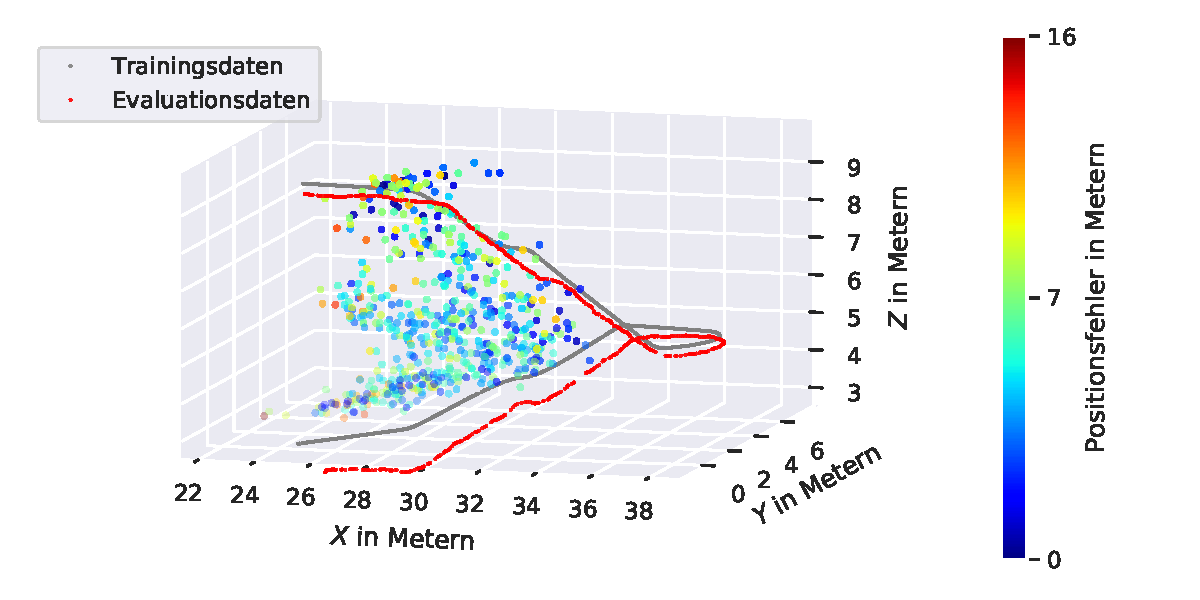
\includegraphics[width=1.0\linewidth]{images/results/hs_down/resultsfig_3.pdf} }\\
		\subcaption{} \label{subfig:hs_down_fig5} & \imagetop{ 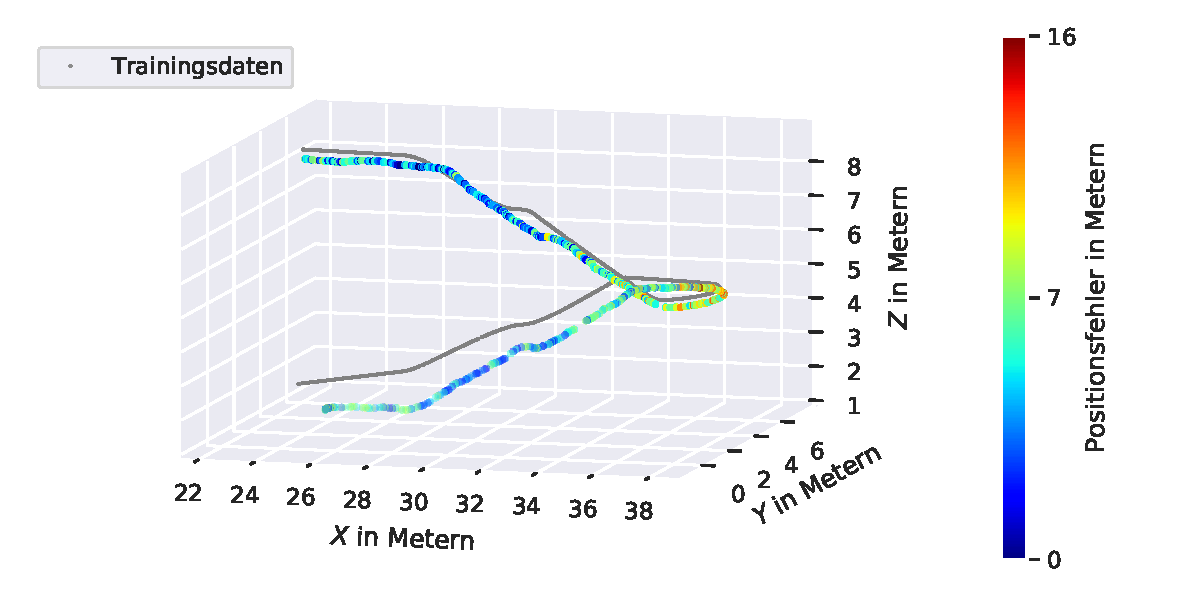
\includegraphics[width=1.0\linewidth]{images/results/hs_down/resultsfig_5.pdf} }\\
		\subcaption{} \label{subfig:hs_down_fig7} & \imagetop{ 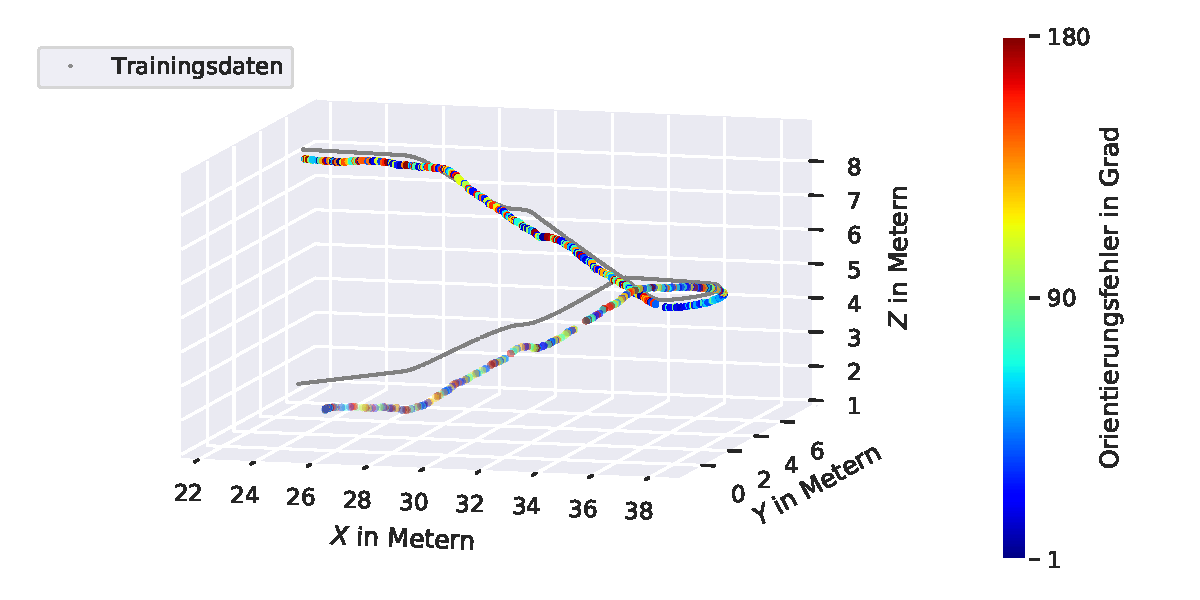
\includegraphics[width=1.0\linewidth]{images/results/hs_down/resultsfig_7.pdf} }\\
	\end{tabularx}
	\caption{Visualisierung der Evaluationsergebnisse von der Strecke \textit{HS-stairs-up}. Die Evaluation folgte mit den Gradietenbildern der realen Daten auf das mit \textit{grad-cartoon} trainierten Netzwerk. \subref{subfig:hs_down_fig3} illustriert die Positionen auf der xy-Ebene, die von dem KNN bestimmt wurden. Der Positionsfehler in der xy-Ebene und der Orientierungsfehler auf der Gierachse der jeweiligen Evaluationsdaten werden in  \subref{subfig:hs_down_fig5} und  \subref{subfig:hs_down_fig7} dargestellt.}
	\label{fig:result_hs_stairs_down}
\end{figure}





